\documentclass[twoside,single]{lion-msc}

\title{Summer Research Internship 2017}
\author{Mudit Garg}

\affiliation{Indian Institute of Technology Delhi}   % this is the default value
%\affiliation{Instituut-Lorentz, Leiden University}                     % for theoretical physics

%\affiliation{Huygens-Kamerlingh Onnes Laboratorium, Universiteit Leiden}   % experimental physics in Dutch
%\affiliation{Instituut-Lorentz, Universiteit Leiden}                       % theoretical physics in Dutch
\id{Senior Undergraduate}
\address{New Delhi, India, 110016}               % default address - uncomment if need be

% \newdate{date}{\day}{\month}{\year}           % definition of time and date using datetime package
%\newdate{date}{27}{08}{2010}
%\date{\displaydate{date}}

\studentid{May-July 2017}                           % check you student ID, LaTeX does not do this
\abstract{}     % limit your self to 1/2 page or 500 words
\supervisor{Prof. Dr. Michel Orrit}                         % Note that this should be a LION staff member!
\dsupervisor{Biswajit Pradhan}                      % This could be a LION staff member or your external supervisor

\degree{Reserach Internship}                     % The default option is "Bachelor of Science", change if needed


\major{Single-Molecule Group,LION}                  % The default option is "Physics", change if needed
%\major{Physics and Mathematics}

% optional cover picture - should be jpg or pdf
\coverpicture{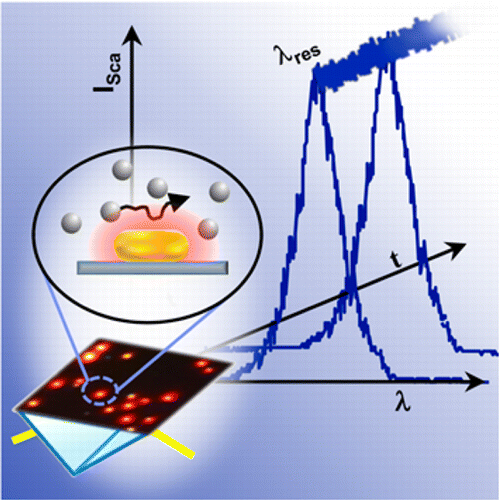
\includegraphics[width=8cm]{1.png}}

% Use this to make hyperlinks visible in the document.
% \hypersetup{colorlinks=true}

% ---------------------------------------------------------------- My defintions!
% \renewcommand{\vec}[1] {\ensuremath{ \overrightarrow{ #1 } }}
\renewcommand{\vec}[1] {\ensuremath{ \mathbf{ #1 } }}
% \bra \ket \braket and \proj
\newcommand{\bra}[1]{\ensuremath{\langle #1 \vert}}
\newcommand{\ket}[1]{\ensuremath{\vert #1 \rangle}}
\newcommand{\braket}[2]{\ensuremath{\langle #1 \vert #2 \rangle}}
\newcommand{\proj}[1]{\ensuremath{\vert #1 \rangle \langle #1 \vert}}

\newcommand{\kpar}{\ensuremath{k_\parallel}}
% ----------------------------------------------------------------

% \usepackage{tocloft}
% \renewcommand{\cftchapdotsep}{\cftdotsep}

\begin{document}

% roman numbering in the table of contents section
\pagenumbering{roman}


\maketitle

% Table of contents :  it is a good idea to include this into your thesis
\tableofcontents
\cleardoublepage

% The following list of figures and list of tables are optional. Remove the comments if needed
%\listoffigures
%\newpage

%\listoftables
%\newpage

% in the main part of the document use standard arabic numbers. Page counter resets to 1.
\pagenumbering{arabic}

\chapter{Introduction}

In this Internship I used Fluroscene Spectrscopy to observe the Gold nanorods as they intract with their nearby particles like protein,silica etc.

\section{Getting Started}

Unzip the zip file into a directory and start with the file minimal.tex. On most systems this should compile if you have the 'lion-msc.cls' file and 'minimal.tex' in the same working directory. 'lion-msc' is based on the report class and any valid option for a report can be passed onto lion-msc. In addition, lion-msc uses several additional packages. Most modern \LaTeX systems have features that allow you to automatically get missing files if your computer is connected to the internet.

A minimal \LaTeX document that should compile with pdf\LaTeX is the following (I called this file 'minimal.tex')

\begin{verbatim}
\documentclass[twoside,single]{lion-msc}

\title{Title}
\author{A. Uthor}

\begin{document}

\maketitle

\chapter{Chapter 1}

Here you type the text for the first chapter of
your thesis.

\end{document}
\end{verbatim}

If problems arise at this point check if you compile \LaTeX directly to pdf. The older route that converts tex files to dvi files and then to postscript is not supported. It is very unlikely that this will be supported in the future.

If problems persist check if you have all necessary files in the right location, most notably 'lion-msc.cls' and 'logo-leidenuniv.pdf'. If you placed the files in some standard location for your tex installation make sure that your installation knows about these files. A quicker, more fail-safe way around this is to place these files in the same working directory as the \LaTeX file that you are trying to compile.

Once you have made these steps take a look at lion-msc.tex as it contains a more complete template that shows how to use the lion-msc documentclass.

\subsection{Files in this package}

The files included with this package are the following:

\vskip 1em

\begin{tabular}{l l}
\hline
\textbf{lion-msc.cls}        & documentclass file \\
\textbf{logo-leidenuniv.pdf} & PDF file with logo of Leiden University. \\
                             & This file is required by the document class \\
\textbf{lion-msc.bst}        & bibliography style file that can be used with bibtex \\
\textbf{lion-msc.layout}     & layout file used for integration with LyX environment \\
\textbf{minimal.tex}         & Minimal \LaTeX file demonstrating the use of \\
                             & lion-msc.cls \\
\textbf{AlexanderPRA.tex}    & \LaTeX file used as an example of a Master Thesis \\
\textbf{lion-msc.tex}        & This file \\
\textbf{lion-msc.pdf}        & PDF file of the compiled version of lion-msc.tex \\
\textbf{thesisstyle.jpg}     & Image used for the cover \\
\textbf{Fig1.png}            & Figure used in AlexanderPRA.tex \\
\textbf{Fig2.png}            & Figure used in AlexanderPRA.tex \\
\textbf{Fig3a.png}           & Figure used in AlexanderPRA.tex \\
\textbf{Fig3b.png}           & Figure used in AlexanderPRA.tex \\
\textbf{Fig4.png}            & Figure used in AlexanderPRA.tex \\
\textbf{4photon.bib}         & BibTeX database file for AlexanderPRA.tex \\
\hline
\end{tabular}

\section{List of available commands and options}

This section gives an overview of special commands and options that are defined through this documentclass. You can use these to change the appearance of your thesis and to include all necessary information.

\subsection{lion-msc options}

Lion-msc inherits and passes its options to the report class. By default the class uses [a4paper, 12pt, fleqn]. If desired this can be passed on by including valid report class options to the options of lion-msc.

\begin{tabular}{l l}
\hline
\textbf{double}        & (default) double line spacing, useful for drafts \\
\textbf{single}        & single line spacing. This looks better in the final version \\
\hline
\end{tabular}

\subsection{Specific lion-msc commands}

With the lion-msc documentclass most of the required information is entered in the preamble of the \LaTeX document (i.e. before $\backslash$begin\{document\}). This information is made visible by using the $\backslash$maketitle command. This should be the first command after $\backslash$begin\{document\}.

Note that you have to fill out the required options. If you leave these empty, instructions will appear in red on the title page. Most of these commands are quite flexible. For instance you can insert newline characters ($\backslash \backslash$) in the affiliation command. This is practical if you do a project outside LION.

\begin{tabular}{l l}
\hline
\textbf{$\backslash$author}       & (required) Defines the author  \\
\textbf{$\backslash$title}        & (required) Defines the title of your thesis \\
\textbf{$\backslash$abstract}     & (required) Provide your abstract here, \\
                                  & making sure that it fits on the page.\\
\textbf{$\backslash$affiliation}  & Sets the affiliation to something else than \\
                                  & the default value. \\
\textbf{$\backslash$address}      & Use this to change the default address if needed. \\
\textbf{$\backslash$studentid}    & (required) enter your student ID (studentnummer) \\
\textbf{$\backslash$supervisor}   & (required) provide a valid supervisor. This should \\
                                  & be a staff member of the Leiden Physics Department \\
\textbf{$\backslash$corrector}    & (required) provide the name of the 2$^{nd}$ dsupervisor. \\
                                  & This could be an external supervisor. \\
\textbf{$\backslash$degree}       & (optional) Default is "Bachelor of Science"\\
                                  & Use this to change the default value. \\
\textbf{$\backslash$major}        & (optional) Default is "Physics" \\
                                  & Use this to change the default value. \\
\textbf{$\backslash$coverpicture} & (optional) Insert a cover picture on the first page \\
                                  & Usage: \\
                                  & $\backslash$coverpicture\{$\backslash$includegraphics[width=13cm]\{picture.jpg\}\} \\
\hline
\end{tabular}

Note that these commands are highly flexible and a bit a \LaTeX knowledge will allow you to make all kinds of smart modifications. A common, and reasonable desire is to give credit to the PhD student or postdoc that guided you during the project. You can do this by trying the following code: \\
$\backslash$supervisor\{PhD student $\backslash \backslash$ $\backslash$hspace*\{$\backslash$fill\}Supervisor\}.\\
Note that you should always have a staff member from Leiden as your supervisor because this person is authorized to give you the final grade.

\subsection{Packages and additional styling tips}

This documentclass uses a number of standard packages, such as amsmath, amssymb for extra functions and symbols to display math and the graphicx package to display graphics in the document. It uses the natbib package to deal with references to automatically sort and compress multiple references. I do not recommend making changes to this in the document preamble. In particular the interplay between natbib and the bibliography style can give very unexpected results.

The default configuration also uses the hyperref package to create a pdf with hyperlinks. The links are hidden so that the text looks normal; try clicking one of the references or in the table of contents and you will see that you are automatically brought to the appropriate reference or section.

The use of packages inside the documentclass can cause an error when you try to use a package within your \LaTeX document. This typically happens when both the documentclass and your own \LaTeX document use some options. There is a $\backslash$PassOptionsToPackage command that you can use before the $\backslash$documentclass to try to pass the desired option to the package.

\subsubsection{Headers with fancyhdr}
The headers and footers on each page contain some useful info. This is done using the \verb"fancyhdr" package. You can change the appearance of these by using the $\backslash$fancyhead and $\backslash$fancyfoot commands. See the \verb"fancyhdr" documentation for details. You can also open lion-msc.cls in a text editor and look for these commands. You can place your own commands before the $\backslash$begin\{document\} command in your \LaTeX file. The grey text at the bottom with date and time is there to help you and your supervisor to keep track of the version, so that we do not end up correcting an old version. It may look somewhat strange in the final version and can be removed by using\\
$\backslash$fancyfoot[CE,CO]\{\}.

\subsubsection{Table of contents styling}

Some people may want to get the original dots back into the table of contents. There is an old-fashioned way of doing this without extra packages. Insert the following in the document preamble. The separation of 4.5 is the default value and can be changed to tune the spacing between dots.
\begin{verbatim}
\makeatletter
\renewcommand\@dotsep{4.5}
\makeatother
\end{verbatim}
An alternative is to use the \verb"tocloft" package that offers additional styling options. Insert the following to use this package. (Suggestion by Casper Remeijer)
\begin{verbatim}
\usepackage{tocloft}
\renewcommand{\cftchapdotsep}{\cftdotsep}
\end{verbatim}

\subsubsection{Subfigures}

It can be quite useful to have multiple figures next to each other. This can be done with the \verb"subcaption" package. (Suggestion by Casper Remeijer)

\begin{verbatim}
\usepackage[labelformat=simple,justification=centering]{subcaption}
\renewcommand\thesubfigure{(\alph{subfigure})}
\end{verbatim}

\subsubsection{Typesetting of units}

Some people rely on a package called 'siunitx' to deal with the correct typesetting of units in the SI system. The following commands could be added 
to the document preamble. (Suggestion by Casper Remeijer)

\begin{verbatim}
\usepackage{siunitx}
\sisetup{separate-uncertainty = true, multi-part-units = single, inter-unit-product = \ensuremath { { } \cdot { } }} 
    % use \pm symbol for uncertainty values, don't repeat the unit, unit multiplication is indicated by means of a half-height dot
\end{verbatim}

\subsubsection{Indentation of paragraphs}

Some people do not like the standard LaTeX indentation at the beginning of the paragraph. This can be changed using the parskip package

\begin{verbatim}
\usepackage{parskip}
\end{verbatim}

\section{Using LyX}

Lyx is a powerfull visual editor that used LateX for typesetting. It exports .tex files that can be submitted to journals. Specifically the visual formula editor is very usefull. It also support track-changes, which is very usefull when collaborating. Some people do not like LyX.

\subsection{Installation}

In order to use the lion-msc style in LyX, the latex style should be installed systemwide. With miktex this is done automatically. Now identify the lion-msc.layout file. It might be located at "c:{\textbackslash}program files{\textbackslash}miktex{\textbackslash}doc{\textbackslash}lion-msc".

The next thing to do is to set the document class to a local layout and choose for the
\emph{lion-msc.layout} file:

Documents $\rhd$ Settings $\rhd$ Document Class $\rhd$ Local-layout

\chapter{Mathematical model}

\chapter{Results and Discussion}
%\appendix
%\include{appa}
\

\bibliographystyle{lion-msc}
\bibliography{4photon}

\end{document}

